\chapter{Lookup}
\blindtext

Dieser Absatz wird zitiert von \citep{Heo2015Control}

Dieser Absatz ist ein bisschen Code
\lstset{language=java, caption=Deklarieren von Variablen in Java }
\begin{lstlisting}

	int i = 0;
	int a = 5;
	int c = a + i;
	//c = 5;
	System.out.println(c);
\end{lstlisting}

\blindtext

\fref{tab:Testtable} ist eine Tabelle mit booktabs und referenziert diese \\
\begin{table}[h]
	\begin{center}
		\begin{tabular}{lcr}
			\toprule
			Spalte 1 & Spalte 2 & Spalte 3 \\
			\midrule
			1 & 2 & 3 \\
			4 & 5 & 6 \\
			\bottomrule
		\end{tabular}
	\end{center}
	\caption{Testtabelle ohne Inhalt}
	\label{tab:Testtable}
\end{table}

\fref{fig:tikzuml} wurde mit tikz gezeichnet\\

\begin{figure}[h]
	\centering
	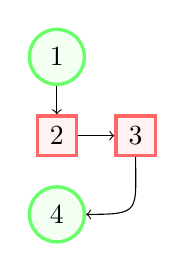
\begin{tikzpicture}[
	roundnode/.style={circle, draw=green!60, fill=green!5, very thick, minimum size=7mm},
	squarenode/.style={rectangle, draw=red!60, fill=red!5, very thick, minimum size=5mm},
	]
	
	%Nodes
	\node[squarenode]		(main)							{2};
	\node[roundnode]		(upper)	[above of=main]		{1};
	\node[squarenode]		(right)	[right of=main]		{3};
	\node[roundnode]		(lower)	[below of=main]		{4};
	
	%Lines
	\draw[->](upper.south) -- (main.north);
	\draw[->](main.east) -- (right.west);
	\draw[->](right.south) .. controls +(down:7mm) and +(right:7mm) .. (lower.east);
	
	\end{tikzpicture}
	\caption{tikz Demo Zeichnung, kann so genutzt werden für UML}
	\label{fig:tikzuml}
\end{figure}

Dieser Absatz verweist auf das Glossar
\gls{acr-k8} \emph{siehe} \gls{gls-k8}

\begin{tabular}{|c|c|c|}
	\hline 
	\cellcolor{green} 1 & \cellcolor{red} 2 & \cellcolor{yellow} 3\\
	\hline 
\end{tabular} 

